% =============================================================================
% GitLab CI/CD Pipeline Infrastructure — Global Workflow
% Standalone Technical Reference Document
% =============================================================================
\documentclass[11pt,letterpaper,twoside]{article}

% --- Page geometry ---
\usepackage[
  top=1in, bottom=1in, left=1in, right=1in,
  headheight=14pt
]{geometry}

% --- Fonts and encoding ---
\usepackage[T1]{fontenc}
\usepackage[utf8]{inputenc}
\usepackage{lmodern}
\usepackage{microtype}

% --- Color ---
\usepackage[dvipsnames,svgnames,table]{xcolor}
\definecolor{noaablue}{HTML}{003087}
\definecolor{noaadarkblue}{HTML}{1e293b}
\definecolor{gitlabpurple}{HTML}{7c3aed}
\definecolor{vlabgreen}{HTML}{16a34a}
\definecolor{triggerorg}{HTML}{ea580c}
\definecolor{heragray}{HTML}{64748b}
\definecolor{lightbg}{HTML}{f8fafc}
\definecolor{codebg}{HTML}{f1f5f9}
\definecolor{notebg}{HTML}{eff6ff}
\definecolor{importbg}{HTML}{fef2f2}
\definecolor{stagebuild}{HTML}{ede9fe}
\definecolor{stagesetup}{HTML}{dbeafe}
\definecolor{stagerun}{HTML}{dcfce7}
\definecolor{stagefinal}{HTML}{fff7ed}

% --- Headers and footers ---
\usepackage{fancyhdr}
\pagestyle{fancy}
\fancyhf{}
\fancyhead[LE,RO]{\thepage}
\fancyhead[RE]{\textit{GitLab CI/CD Pipeline Infrastructure}}
\fancyhead[LO]{\textit{Global Workflow — NOAA/EMC}}
\renewcommand{\headrulewidth}{0.4pt}
\fancypagestyle{plain}{%
  \fancyhf{}%
  \fancyfoot[C]{\thepage}%
  \renewcommand{\headrulewidth}{0pt}%
}

% --- Section formatting ---
\usepackage{titlesec}
\titleformat{\section}
  {\normalfont\Large\bfseries\color{noaablue}}{\thesection}{1em}{}
\titleformat{\subsection}
  {\normalfont\large\bfseries\color{noaadarkblue}}{\thesubsection}{1em}{}
\titleformat{\subsubsection}
  {\normalfont\normalsize\bfseries\color{noaadarkblue}}{\thesubsubsection}{1em}{}

% --- Tables ---
\usepackage{longtable}
\usepackage{tabularx}
\usepackage{booktabs}
\usepackage{colortbl}

% --- Lists ---
\usepackage{enumitem}

% --- Code listings ---
\usepackage{listings}
\lstset{
  basicstyle=\ttfamily\small,
  backgroundcolor=\color{codebg},
  frame=single,
  framerule=0.4pt,
  rulecolor=\color{gray!40},
  breaklines=true,
  breakatwhitespace=false,
  showstringspaces=false,
  columns=fullflexible,
  keepspaces=true,
  xleftmargin=4pt,
  xrightmargin=4pt,
  aboveskip=8pt,
  belowskip=8pt,
}
\lstdefinestyle{yaml}{
  language={},
  morekeywords={experiment,net,mode,app,resdetatmos,idate,edate,workflow,engine,rocoto,maxtries,extends,variables,machine,tags,parallel,matrix,needs,rules,if,caseName},
  keywordstyle=\color{noaablue}\bfseries,
  stringstyle=\color{DarkGreen},
  commentstyle=\color{gray},
  morecomment=[l]{\#},
  morestring=[b]",
  morestring=[b]',
}
\lstdefinestyle{bash}{
  language=bash,
  keywordstyle=\color{noaablue}\bfseries,
  stringstyle=\color{DarkGreen},
  commentstyle=\color{gray}\itshape,
}

% --- TikZ for diagrams ---
\usepackage{tikz}
\usetikzlibrary{
  positioning,
  arrows.meta,
  shapes.geometric,
  shapes.multipart,
  fit,
  calc,
  backgrounds,
  shadows,
  decorations.pathreplacing,
  decorations.markings,
  patterns
}

% --- Floats ---
\usepackage{float}

% --- Adjustbox for fitting wide content ---
\usepackage[export]{adjustbox}

% --- tcolorbox for styled boxes ---
\usepackage[skins,breakable]{tcolorbox}

% --- Hyperlinks (must be last of these) ---
\usepackage{hyperref}
\hypersetup{
  colorlinks=true,
  linkcolor=noaablue,
  urlcolor=gitlabpurple,
  citecolor=noaablue,
  pdfauthor={NOAA/EMC Global Workflow CI/CD Team},
  pdftitle={GitLab CI/CD Pipeline Infrastructure},
  pdfsubject={Technical Reference for Global Workflow CI/CD},
  bookmarksnumbered=true,
}

% --- Custom environments for notes/warnings ---
\newtcolorbox{notebox}{
  colback=notebg, colframe=noaablue!60, boxrule=0.6pt,
  left=8pt, right=8pt, top=6pt, bottom=6pt,
  fonttitle=\bfseries\color{noaablue},
  title=Note, rounded corners, arc=3pt,
  before upper={\color{noaadarkblue}}
}

\newtcolorbox{importantbox}{
  colback=importbg, colframe=red!50!black, boxrule=0.6pt,
  left=8pt, right=8pt, top=6pt, bottom=6pt,
  fonttitle=\bfseries\color{red!70!black},
  title=Important, rounded corners, arc=3pt,
  before upper={\color{noaadarkblue}}
}

% --- Document metadata ---
\title{%
  \vspace{-0.5in}
  {\color{noaablue}\rule{\linewidth}{2pt}}\\[12pt]
  {\Huge\bfseries\color{noaadarkblue} GitLab CI/CD Pipeline\\[4pt] Infrastructure}\\[10pt]
  {\Large\color{heragray} Global Workflow Technical Reference}\\[12pt]
  {\color{noaablue}\rule{\linewidth}{2pt}}
}
\author{%
  NOAA / NWS / NCEP / EMC\\[2pt]
  {\normalsize Global Workflow Development Team}\\[2pt]
  {\small\texttt{https://github.com/NOAA-EMC/global-workflow}}
}
\date{March 2026}

% =============================================================================
\begin{document}
\maketitle
\thispagestyle{plain}

\begin{abstract}
\noindent
This document provides a comprehensive, standalone technical reference for the
GitLab CI/CD pipeline infrastructure used by the NOAA/EMC global-workflow
project. It covers the repository mirroring strategy between GitHub and GitLab,
the pipeline architecture and configuration, the GitLab runner deployment on
NOAA's Research and Development High-Performance Computing Systems (RDHPCS),
nightly pipeline operations, and the day-to-day maintenance procedures that
keep the system operational. All architectural diagrams are reproduced as
native vector figures for print-quality output.
\end{abstract}

\tableofcontents
\newpage

% =============================================================================
\section{Overview}
\label{sec:overview}
% =============================================================================

The global-workflow CI/CD system uses \textbf{GitLab CI/CD} as the execution
engine for continuous integration testing across NOAA's Research and Development
High-Performance Computing Systems (RDHPCS). GitHub remains the
\textbf{authoritative repository} where all development, code review, and pull
request activity occurs.

The fundamental challenge this infrastructure solves is that NOAA's HPC systems
(Hera, Gaea, Orion, Hercules, Ursa) are not directly accessible from GitHub
Actions runners. By mirroring the repository to GitLab and placing GitLab
runners directly on those HPC systems, the project gains the ability to build
and test the workflow in the same environments where it will be deployed
operationally.

\subsection{Key Design Principles}
\label{sec:design-principles}

\begin{itemize}[leftmargin=1.5em]
  \item \textbf{GitHub is authoritative} --- All development happens on GitHub
    (\url{https://github.com/NOAA-EMC/global-workflow}). GitLab is used solely
    as a CI execution platform.
  \item \textbf{Two-tier mirroring} --- A licensed GitLab instance performs the
    pull mirror from GitHub, and subsequently push mirrors to the NOAA community
    GitLab instance.
  \item \textbf{HPC-native testing} --- Runners execute directly on the target
    HPC nodes, ensuring tests build and run against the real Spack-Stack
    software environment.
  \item \textbf{Multi-modal pipelines} --- The system supports both
    comprehensive end-to-end experiment cases and fast CTest-based functional
    checks.
  \item \textbf{GitHub feedback loop} --- Pipeline results flow back to GitHub
    through PR labels, PR comments (including error log gists), and status
    badges.
\end{itemize}


% =============================================================================
% FIGURE 1: High-Level Architecture
% =============================================================================
\begin{figure}[H]
\centering
\begin{adjustbox}{max width=\textwidth}
\begin{tikzpicture}[
  >=Stealth,
  node distance=0.8cm and 1.2cm,
  repo/.style={
    rectangle, rounded corners=6pt, minimum width=4.6cm, minimum height=2.4cm,
    text width=4.2cm, align=center, font=\small, draw, line width=1pt,
    fill=white, drop shadow={shadow xshift=1pt, shadow yshift=-1pt,
    fill=black!15}
  },
  stage/.style={
    rectangle, rounded corners=4pt, minimum width=2.6cm, minimum height=1.7cm,
    text width=2.3cm, align=center, font=\scriptsize, draw, line width=0.8pt
  },
  runner/.style={
    rectangle, rounded corners=4pt, minimum width=2.4cm, minimum height=1.8cm,
    text width=2.1cm, align=center, font=\scriptsize, draw=vlabgreen,
    line width=1pt, fill=white, drop shadow={shadow xshift=1pt,
    shadow yshift=-1pt, fill=black!10}
  },
  mirrortag/.style={
    rectangle, rounded corners=3pt, minimum height=0.45cm,
    font=\scriptsize\bfseries, inner sep=3pt
  },
  every label/.style={font=\scriptsize\color{heragray}}
]

% --- Row 1: Repositories ---
\node[repo, draw=noaadarkblue, fill=white] (github) {
  \textbf{\color{noaadarkblue}GitHub}\\[1pt]
  {\color{noaadarkblue}\footnotesize(Authoritative)}\\[4pt]
  {\scriptsize\texttt{NOAA-EMC/}}\\[-1pt]
  {\scriptsize\texttt{global-workflow}}\\[3pt]
  {\tiny\color{heragray}Development\,\textbullet\,Code Review}\\[-1pt]
  {\tiny\color{heragray}PRs\,\textbullet\,Issues\,\textbullet\,Releases}
};

\node[repo, draw=gitlabpurple, right=2.2cm of github] (licensed) {
  \textbf{\color{gitlabpurple}Licensed GitLab}\\[1pt]
  {\color{gitlabpurple}\footnotesize Instance}\\[4pt]
  {\scriptsize GitLab Premium}\\[3pt]
  {\tiny\color{heragray}Pull Mirror\,\textbullet\,Push Mirror}\\[-1pt]
  {\tiny\color{heragray}Mirroring Only (No CI)}
};

\node[repo, draw=vlabgreen, right=2.2cm of licensed] (vlab) {
  \textbf{\color{vlabgreen}VLab Community}\\[1pt]
  {\color{vlabgreen}\footnotesize GitLab}\\[4pt]
  {\scriptsize\texttt{vlab.noaa.gov/}}\\[-1pt]
  {\scriptsize\texttt{gitlab-community}}\\[3pt]
  {\tiny\color{heragray}CI/CD Pipeline Execution}\\[-1pt]
  {\tiny\color{heragray}Runners\,\textbullet\,NOAA-Wide Access}
};

% --- Mirror arrows ---
\draw[->, noaablue, line width=1.8pt]
  (github.east) -- node[mirrortag, above, fill=blue!8, text=noaablue]
  {PULL} (licensed.west);
\draw[->, vlabgreen, line width=1.8pt]
  (licensed.east) -- node[mirrortag, above, fill=green!8, text=vlabgreen]
  {PUSH} (vlab.west);

% --- Feedback loop (top) ---
\draw[->, gray, dashed, line width=0.9pt]
  (vlab.north) .. controls +(0,1.1) and +(0,1.1) .. 
  node[above, font=\tiny\color{heragray}, pos=0.5]
  {Labels\,\textbullet\,Comments\,\textbullet\,Badges} (github.north);

% --- GitHub Actions trigger (bottom curve) ---
\draw[->, triggerorg, densely dashed, line width=1.2pt]
  (github.south) .. controls +(0,-1.2) and +(0,-1.2) ..
  node[below, font=\tiny\bfseries\color{triggerorg}, pos=0.5]
  {GitHub Actions Trigger} (vlab.south);

% --- Row 2: Pipeline Stages ---
\node[below=2.4cm of licensed, font=\small\bfseries\color{gitlabpurple}]
  (pipelabel) {GitLab CI/CD Pipeline Stages};

\node[stage, fill=stagebuild, draw=gitlabpurple,
  below left=0.3cm and 2.8cm of pipelabel] (build) {
  \textbf{\color{gitlabpurple}1.\,Build}\\[2pt]
  Clone \& checkout PR\\
  Compile codebase\\
  Link workflow
};
\node[stage, fill=stagesetup, draw=noaablue, right=0.3cm of build] (setup) {
  \textbf{\color{noaablue}2.\,Setup}\\[2pt]
  Create experiments\\
  or CMake/CTest\\
  configuration
};
\node[stage, fill=stagerun, draw=vlabgreen, right=0.3cm of setup] (run) {
  \textbf{\color{vlabgreen}3.\,Run Tests}\\[2pt]
  Rocoto experiments\\
  or CTest execution\\
  Monitor \& report
};
\node[stage, fill=stagefinal, draw=triggerorg, right=0.3cm of run] (finalize) {
  \textbf{\color{triggerorg}4.\,Finalize}\\[2pt]
  Update PR labels\\
  Manage nightlies\\
  Update badges
};

% Stage arrows
\draw[->, gray, line width=1pt] (build.east) -- (setup.west);
\draw[->, gray, line width=1pt] (setup.east) -- (run.west);
\draw[->, gray, line width=1pt] (run.east) -- (finalize.west);

% Connect VLab to pipeline
\draw[->, gray, line width=1pt] (vlab.south) -- ++(0,-0.6) -| (pipelabel.north);

% --- Pipeline modalities box ---
\node[rectangle, rounded corners=4pt, draw=Goldenrod, fill=yellow!5,
  line width=0.8pt, text width=3.4cm, align=left, font=\scriptsize,
  right=0.4cm of finalize, yshift=-0.1cm] (modes) {
  \textbf{\color{Goldenrod}Pipeline Modalities}\\[3pt]
  {\color{gitlabpurple}\textbullet}\;\textbf{PR Cases}\\
  {\tiny Full Rocoto experiments}\\[2pt]
  {\color{noaablue}\textbullet}\;\textbf{CTests}\\
  {\tiny Fast CMake/CTest checks}
};

% --- Row 3: RDHPCS Runners ---
\begin{scope}[on background layer]
  \node[rectangle, rounded corners=6pt, fill=green!3, draw=vlabgreen,
    dashed, line width=0.8pt, inner sep=10pt,
    fit=(build)(finalize)(modes), yshift=-3.2cm,
    minimum width=16cm, minimum height=2.6cm] (runnerbox) {};
\end{scope}

\node[font=\small\bfseries\color{vlabgreen},
  anchor=north] at ([yshift=-2.3cm]$(build.south)!0.5!(finalize.south)$)
  (runnerlabel) {RDHPCS GitLab Shell Runners};

\node[font=\tiny\color{vlabgreen}, below=0pt of runnerlabel]
  (runnersub) {Deployed via \texttt{launch\_gitlab\_runner.sh} on each HPC system};

\node[runner, below=0.35cm of runnersub, xshift=-5.6cm] (hera) {
  \textbf{\color{vlabgreen}Hera}\\[1pt]
  {\tiny NOAA RDHPCS}\\
  {\tiny 17 test cases}\\
  {\tiny\color{heragray}Tag: \texttt{hera}}
};
\node[runner, right=0.25cm of hera] (gaea) {
  \textbf{\color{vlabgreen}Gaea\,C6}\\[1pt]
  {\tiny DOE/ORNL}\\
  {\tiny 15 test cases}\\
  {\tiny\color{heragray}Tag: \texttt{gaeac6}}
};
\node[runner, right=0.25cm of gaea] (orion) {
  \textbf{\color{vlabgreen}Orion}\\[1pt]
  {\tiny MSU RDHPCS}\\
  {\tiny 8 test cases}\\
  {\tiny\color{heragray}Tag: \texttt{orion}}
};
\node[runner, right=0.25cm of orion] (herc) {
  \textbf{\color{vlabgreen}Hercules}\\[1pt]
  {\tiny MSU RDHPCS}\\
  {\tiny 10 test cases}\\
  {\tiny\color{heragray}Tag: \texttt{hercules}}
};
\node[runner, right=0.25cm of herc] (ursa) {
  \textbf{\color{vlabgreen}Ursa}\\[1pt]
  {\tiny NOAA RDHPCS}\\
  {\tiny 17 test cases}\\
  {\tiny\color{heragray}Tag: \texttt{ursa}}
};

% Connect pipeline to runners
\foreach \r in {hera,gaea,orion,herc,ursa} {
  \draw[vlabgreen, dashed, line width=0.6pt]
    ([yshift=-0.2cm]run.south) -- (\r.north);
}

\end{tikzpicture}
\end{adjustbox}
\caption{High-level CI/CD architecture showing repository mirroring,
  pipeline stages, and RDHPCS runner deployment.}
\label{fig:architecture}
\end{figure}


% =============================================================================
\section{Repository Mirroring: GitHub to GitLab}
\label{sec:mirroring}
% =============================================================================

Because GitHub is the authoritative source of truth and GitLab is the CI
execution platform, a reliable synchronization mechanism is required. The
global-workflow project uses a \textbf{two-stage mirroring strategy} involving
two GitLab instances.

\subsection{Pull Mirroring (Licensed GitLab Instance)}
\label{sec:pull-mirror}

The first stage uses \textbf{pull mirroring}, a feature that is only available
on licensed (paid) tiers of GitLab (Premium or Ultimate). A single licensed
GitLab instance is configured to pull from the authoritative GitHub repository:

\begin{table}[H]
\centering
\caption{Pull Mirror Configuration}
\label{tab:pull-mirror}
\begin{tabularx}{\linewidth}{lX}
\toprule
\textbf{Setting} & \textbf{Value} \\
\midrule
Source repository & \texttt{https://github.com/NOAA-EMC/global-workflow.git} \\
Direction & Pull \\
Scope & All branches \\
Sync frequency & Automatic (every few minutes) \\
\bottomrule
\end{tabularx}
\end{table}

The licensed instance's sole purpose is \textbf{mirroring} --- it does not run
any CI/CD pipelines itself. Its pull mirror keeps the GitLab copy synchronized
with GitHub, and its push mirror (described below) propagates changes onward.

\begin{notebox}
Pull mirroring is an \textbf{advanced feature} available only on licensed
instances of GitLab (Premium tier and above). It is not available on GitLab
Community Edition (CE) or the free tier. This is why a separate licensed
instance is required for the first stage of the mirror chain.
\end{notebox}

\subsection{Push Mirroring (Community GitLab at VLab)}
\label{sec:push-mirror}

The second stage uses \textbf{push mirroring} from the licensed GitLab instance
to the NOAA community GitLab instance hosted at VLab:

\begin{table}[H]
\centering
\caption{Push Mirror Configuration}
\label{tab:push-mirror}
\begin{tabularx}{\linewidth}{lX}
\toprule
\textbf{Setting} & \textbf{Value} \\
\midrule
Target repository & {\small\texttt{https://vlab.noaa.gov/gitlab-community/\allowbreak NWS/Operations/NCEP/EMC/\allowbreak global-workflow.git}} \\
Direction & Push \\
Scope & All branches \\
Sync frequency & Automatic (every few minutes) \\
\bottomrule
\end{tabularx}
\end{table}

The VLab community GitLab instance is where the \textbf{CI/CD pipelines
actually execute}. GitLab runners deployed on RDHPCS systems register against
this instance, and all pipeline stages (build, setup, test, finalize) run here.
This instance also provides the broader NOAA user community with read access to
the repository.

\subsection{Mirror Chain Summary}
\label{sec:mirror-summary}

% --- Figure 2: Mirror Chain ---
\begin{figure}[H]
\centering
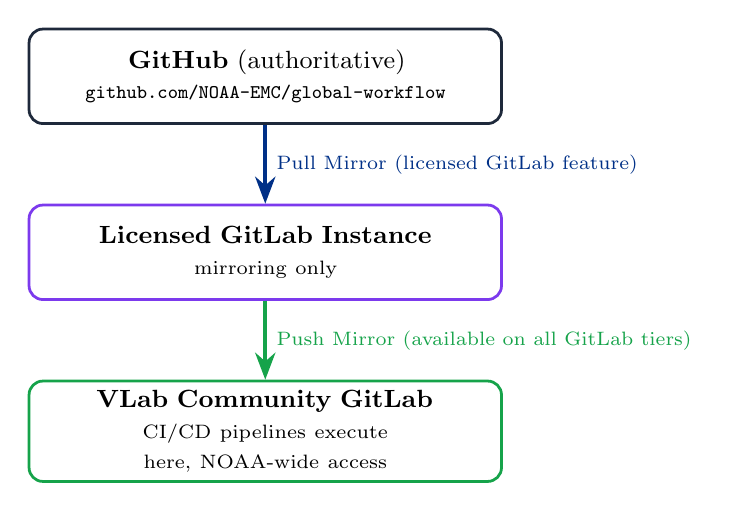
\begin{tikzpicture}[
  >=Stealth,
  chainbox/.style={
    rectangle, rounded corners=5pt, minimum width=6cm, minimum height=1.2cm,
    text width=5.6cm, align=center, font=\small, draw, line width=1pt,
    fill=white
  }
]

\node[chainbox, draw=noaadarkblue] (gh) {
  \textbf{GitHub} (authoritative)\\
  {\scriptsize\texttt{github.com/NOAA-EMC/global-workflow}}
};
\node[chainbox, draw=gitlabpurple, below=1cm of gh] (lic) {
  \textbf{Licensed GitLab Instance}\\
  {\scriptsize mirroring only}
};
\node[chainbox, draw=vlabgreen, below=1cm of lic] (vl) {
  \textbf{VLab Community GitLab}\\
  {\scriptsize CI/CD pipelines execute here, NOAA-wide access}
};

\draw[->, noaablue, line width=1.5pt] (gh) -- node[right, font=\scriptsize,
  text=noaablue] {Pull Mirror (licensed GitLab feature)} (lic);
\draw[->, vlabgreen, line width=1.5pt] (lic) -- node[right, font=\scriptsize,
  text=vlabgreen] {Push Mirror (available on all GitLab tiers)} (vl);

\end{tikzpicture}
\caption{Complete mirror chain from GitHub to the CI/CD execution environment.}
\label{fig:mirror-chain}
\end{figure}

Both mirrored repositories track \textbf{all branches}, ensuring that any
branch pushed to GitHub (including PR branches fetched during pipeline
execution) is available for CI testing.

\begin{importantbox}
Developers should \textbf{never push directly} to either GitLab instance. All
code changes must flow through GitHub. The GitLab mirrors are read-only copies
maintained by the mirroring configuration.
\end{importantbox}


% =============================================================================
\section{Pipeline Architecture}
\label{sec:pipeline}
% =============================================================================

The pipeline is defined across four YAML configuration files that are included
from the top-level \texttt{.gitlab-ci.yml}:

\begin{table}[H]
\centering
\caption{Pipeline Configuration Files}
\label{tab:pipeline-files}
\begin{tabularx}{\linewidth}{lX}
\toprule
\textbf{File} & \textbf{Purpose} \\
\midrule
\texttt{.gitlab-ci.yml} & Main orchestration: stages, variables, base templates, build template \\
\texttt{dev/ci/gitlab-ci-cases.yml} & Templates for standard experiment test cases (setup, run, finalize) \\
\texttt{dev/ci/gitlab-ci-ctests.yml} & Templates for CTest-based functional testing (CMake/CTest) \\
\texttt{dev/ci/gitlab-ci-hosts.yml} & Host-specific jobs, test matrices, runner tags, and conditional rules \\
\bottomrule
\end{tabularx}
\end{table}

\subsection{Pipeline Stages}
\label{sec:stages}

Every pipeline execution proceeds through four stages in order:

\begin{enumerate}[leftmargin=1.5em]
  \item \textbf{build} --- Clone the repository, checkout the PR branch (if
    applicable), build the codebase via \texttt{ci\_utils.sh build}, and link
    the workflow.
  \item \textbf{setup\_tests} --- Prepare the test environment: create
    experiment directories (PR Cases) or configure the CMake/CTest build
    (CTests).
  \item \textbf{run\_tests} --- Execute the tests: run Rocoto-orchestrated
    experiments (PR Cases) or run \texttt{ctest} with specific labels (CTests).
  \item \textbf{finalize} --- Report results: update GitHub PR labels, manage
    nightly directory symlinks, and update status badges.
\end{enumerate}

% --- Figure 3: Pipeline stages detail ---
\begin{figure}[H]
\centering
\begin{adjustbox}{max width=\textwidth}
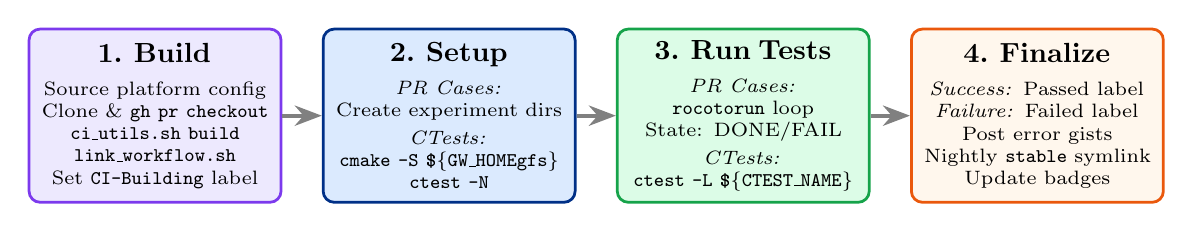
\begin{tikzpicture}[
  >=Stealth,
  sbox/.style={
    rectangle, rounded corners=4pt, minimum width=3.2cm, minimum height=2.2cm,
    text width=2.9cm, align=center, font=\scriptsize, draw, line width=1pt
  }
]

\node[sbox, fill=stagebuild, draw=gitlabpurple] (s1) {
  \textbf{\normalsize 1. Build}\\[4pt]
  Source platform config\\
  Clone \& \texttt{gh pr checkout}\\
  \texttt{ci\_utils.sh build}\\
  \texttt{link\_workflow.sh}\\
  Set \texttt{CI-Building} label
};
\node[sbox, fill=stagesetup, draw=noaablue, right=0.5cm of s1] (s2) {
  \textbf{\normalsize 2. Setup}\\[4pt]
  \textit{PR Cases:}\\
  Create experiment dirs\\[2pt]
  \textit{CTests:}\\
  \texttt{cmake -S \$\{GW\_HOMEgfs\}}\\
  \texttt{ctest -N}
};
\node[sbox, fill=stagerun, draw=vlabgreen, right=0.5cm of s2] (s3) {
  \textbf{\normalsize 3. Run Tests}\\[4pt]
  \textit{PR Cases:}\\
  \texttt{rocotorun} loop\\
  State: DONE/FAIL\\[2pt]
  \textit{CTests:}\\
  \texttt{ctest -L \$\{CTEST\_NAME\}}
};
\node[sbox, fill=stagefinal, draw=triggerorg, right=0.5cm of s3] (s4) {
  \textbf{\normalsize 4. Finalize}\\[4pt]
  \textit{Success:} Passed label\\
  \textit{Failure:} Failed label\\
  Post error gists\\
  Nightly \texttt{stable} symlink\\
  Update badges
};

\draw[->, line width=1.5pt, gray] (s1.east) -- (s2.west);
\draw[->, line width=1.5pt, gray] (s2.east) -- (s3.west);
\draw[->, line width=1.5pt, gray] (s3.east) -- (s4.west);

\end{tikzpicture}
\end{adjustbox}
\caption{Detailed view of the four pipeline stages and their key operations.}
\label{fig:stages-detail}
\end{figure}

\subsection{Pipeline Modalities}
\label{sec:modalities}

The \texttt{PIPELINE\_TYPE} variable controls which testing modality runs.

\subsubsection{PR Cases (\texttt{PIPELINE\_TYPE=pr\_cases})}
\label{sec:pr-cases}

Comprehensive end-to-end experiment testing. Each test case is defined by a YAML
file in \texttt{dev/ci/cases/pr/} that specifies an experiment configuration:

\begin{lstlisting}[style=yaml, caption={Example PR case definition (\texttt{dev/ci/cases/pr/C48\_ATM.yaml})}, label=lst:case-yaml]
# Example: dev/ci/cases/pr/C48_ATM.yaml
experiment:
  net: gfs
  mode: forecast-only
  app: ATM
  resdetatmos: 48
  idate: 2021032312
  edate: 2021032312

workflow:
  engine: rocoto
  rocoto:
    maxtries: 2
\end{lstlisting}

The pipeline creates a full experiment directory, launches Rocoto, and monitors
the workflow to completion. Failures are detected through Rocoto state tracking
and reported back to the GitHub PR with error log gists.

\textbf{Currently defined PR case tests include:}

\begin{itemize}[leftmargin=1.5em, itemsep=1pt]
  \item \texttt{C48\_ATM} --- Atmosphere-only forecast
  \item \texttt{C48\_S2SW} --- Coupled atmosphere-ocean-ice-wave
  \item \texttt{C48\_S2SWA\_gefs} --- GEFS ensemble coupled run
  \item \texttt{C48mx500\_3DVarAOWCDA} --- 3DVar coupled data assimilation
  \item \texttt{C48mx500\_hybAOWCDA} --- Hybrid EnVar coupled data assimilation
  \item \texttt{C96C48\_hybatmDA} --- Hybrid atmosphere-only data assimilation
  \item \texttt{C96C48\_hybatmsnowDA} --- Hybrid atmosphere + snow DA
  \item \texttt{C96C48\_hybatmsoilDA} --- Hybrid atmosphere + soil DA
  \item \texttt{C96\_atm3DVar} --- C96 resolution 3DVar atmosphere
  \item \texttt{C96\_gcafs\_cycled} --- GCAFS cycled system
  \item \texttt{C96mx100\_S2S} --- Seasonal-to-subseasonal coupled
  \item \texttt{C48\_gsienkf\_atmDA} --- GSI ensemble Kalman filter
  \item \texttt{C48\_ufsenkf\_atmDA} --- UFS ensemble Kalman filter
\end{itemize}

See \texttt{dev/ci/gitlab-ci-hosts.yml} for the complete per-machine matrices.

\subsubsection{CTests (\texttt{PIPELINE\_TYPE=ctests})}
\label{sec:ctests}

Fast, focused unit-level testing using the CMake/CTest framework. These tests
exercise individual Rocoto jobs (JJOBS) with predefined, pre-staged input data
and verify their outputs against baselines from nightly stable runs.

The CTest flow:

\begin{enumerate}[leftmargin=1.5em]
  \item \texttt{cmake -S "\$\{GW\_HOMEgfs\}"} --- Configure the CTest build
  \item \texttt{ctest -N} --- List available tests
  \item \texttt{ctest -L "\$\{CTEST\_NAME\}"} --- Run tests matching a specific label
  \item JUnit XML results are published as GitLab artifacts
\end{enumerate}

CTests provide rapid developer feedback (minutes instead of hours) and are
ideal for targeted validation of specific job changes.

\subsection{Per-Host Test Matrices}
\label{sec:host-matrices}

Each HPC platform runs a specific subset of test cases, defined in
\texttt{dev/ci/gitlab-ci-hosts.yml}. The matrices reflect the software and data
availability on each system:

\begin{longtable}{p{2cm}p{12cm}}
\caption{Test Cases by Platform} \label{tab:host-cases} \\
\toprule
\textbf{Platform} & \textbf{Test Cases} \\
\midrule
\endfirsthead
\toprule
\textbf{Platform} & \textbf{Test Cases} \\
\midrule
\endhead
\bottomrule
\endfoot

\textbf{Hera} &
  C48\_ATM, C48\_S2SW, C48\_S2SWA\_gefs,
  C48mx500\_3DVarAOWCDA, C48mx500\_hybAOWCDA,
  C96C48\_hybatmDA, C96C48\_hybatmsnowDA, C96C48\_hybatmsoilDA,
  C96C48\_ufsgsi\_hybatmDA, C96C48\_ufs\_hybatmDA,
  C96C48mx500\_S2SW\_cyc\_gfs, C96\_atm3DVar,
  C96\_gcafs\_cycled, C96\_gcafs\_cycled\_noDA,
  C96mx100\_S2S, C48\_gsienkf\_atmDA, C48\_ufsenkf\_atmDA \\
\midrule

\textbf{Gaea\,C6} &
  C48\_ATM, C48\_S2SW, C48\_S2SWA\_gefs,
  C48mx500\_3DVarAOWCDA, C48mx500\_hybAOWCDA,
  C96C48\_hybatmDA, C96C48\_hybatmsnowDA, C96C48\_hybatmsoilDA,
  C96C48mx500\_S2SW\_cyc\_gfs, C96\_atm3DVar,
  C96\_gcafs\_cycled, C96\_gcafs\_cycled\_noDA,
  C96mx100\_S2S, C48\_gsienkf\_atmDA, C48\_ufsenkf\_atmDA \\
\midrule

\textbf{Orion} &
  C48\_ATM, C48\_S2SW, C48\_S2SWA\_gefs,
  C96C48\_hybatmDA, C96C48mx500\_S2SW\_cyc\_gfs,
  C96\_atm3DVar, C96mx100\_S2S, C96\_gcafs\_cycled \\
\midrule

\textbf{Hercules} &
  C48\_ATM, C48\_S2SW, C48\_S2SWA\_gefs,
  C48mx500\_3DVarAOWCDA, C48mx500\_hybAOWCDA,
  C96C48\_hybatmDA, C96C48mx500\_S2SW\_cyc\_gfs,
  C96\_atm3DVar, C96mx100\_S2S, C96\_gcafs\_cycled \\
\midrule

\textbf{Ursa} &
  C48\_ATM, C48\_S2SW, C48\_S2SWA\_gefs,
  C48mx500\_3DVarAOWCDA, C48mx500\_hybAOWCDA,
  C96C48\_hybatmDA, C96C48\_hybatmsnowDA, C96C48\_hybatmsoilDA,
  C96C48\_ufsgsi\_hybatmDA, C96C48\_ufs\_hybatmDA,
  C96C48mx500\_S2SW\_cyc\_gfs, C96\_atm3DVar,
  C96mx100\_S2S, C96\_gcafs\_cycled, C96\_gcafs\_cycled\_noDA,
  C48\_gsienkf\_atmDA, C48\_ufsenkf\_atmDA \\

\end{longtable}

\subsection{Pipeline Variables}
\label{sec:pipeline-vars}

The following variables control pipeline behavior and can be set from GitLab
scheduled pipelines, GitHub Actions triggers, or the GitLab web UI:

\begin{table}[H]
\centering
\caption{Key Pipeline Variables}
\label{tab:pipeline-vars}
\begin{tabularx}{\linewidth}{llX}
\toprule
\textbf{Variable} & \textbf{Default} & \textbf{Description} \\
\midrule
\texttt{PIPELINE\_TYPE} & \texttt{pr\_cases} & Testing modality: \texttt{pr\_cases} or \texttt{ctests} \\
\texttt{GFS\_CI\_RUN\_TYPE} & \texttt{pr\_cases} & Run classification: \texttt{pr\_cases} or \texttt{nightly} \\
\texttt{RUN\_ON\_MACHINES} & \texttt{all} & Space-separated list of machines or \texttt{all} \\
\texttt{PR\_NUMBER} & \texttt{0} & GitHub PR number (\texttt{0}\,=\,develop branch) \\
\texttt{GITHUB\_COMMIT\_SHA} & (empty) & PR head commit SHA for GitLab native GitHub integration \\
\texttt{GW\_REPO\_URL} & \footnotesize\texttt{...github.com/ NOAA-EMC/...} & Authoritative GitHub repository URL \\
\bottomrule
\end{tabularx}
\end{table}


% =============================================================================
\section{GitHub Actions Integration}
\label{sec:github-actions}
% =============================================================================

Pipelines are triggered from GitHub via the
\texttt{trigger-gitlab-pipelines.yml} workflow in
\texttt{.github/\allowbreak{}workflows/}. This provides a user-friendly
interface for developers to initiate CI testing.

\subsection{Triggering a Pipeline}
\label{sec:triggering}

\begin{enumerate}[leftmargin=1.5em]
  \item Navigate to the \textbf{Actions} tab in the GitHub repository.
  \item Select the \textbf{``Trigger GitLab Pipelines''} workflow.
  \item Click \textbf{``Run workflow''} and configure the inputs:
    \begin{itemize}[leftmargin=1.5em]
      \item \textbf{PR number}: Enter the PR number to test, or \texttt{0} for
        the develop branch.
      \item \textbf{Pipeline Type}: Choose ``PR Cases'' or ``CTests''.
      \item \textbf{Machine checkboxes}: Select which RDHPCS machines to run on
        (Hera, Gaea\,C6, Orion, Hercules, Ursa).
    \end{itemize}
  \item Click \textbf{``Run workflow''} to submit.
\end{enumerate}

The workflow performs the following:

\begin{enumerate}[leftmargin=1.5em]
  \item \textbf{Permission check}: Verifies the triggering user is in the
    \texttt{AUTHORIZED\_GITLAB\_TRIGGER\_USERS} list (stored as a GitHub
    repository variable).
  \item \textbf{Parameter setup}: Resolves the PR head commit SHA, determines
    the pipeline type, and builds the machine selection list.
  \item \textbf{GitLab trigger}: Sends a POST request to the GitLab Pipeline
    Trigger API with all the necessary variables.
  \item \textbf{Label management}: Adds \texttt{CI-<Machine>-Ready} labels to
    the PR on GitHub.
\end{enumerate}

\subsection{Required GitHub Secrets and Variables}
\label{sec:github-secrets}

\begin{table}[H]
\centering
\caption{GitHub Configuration}
\label{tab:github-config}
\begin{tabularx}{\linewidth}{llX}
\toprule
\textbf{Name} & \textbf{Type} & \textbf{Description} \\
\midrule
\texttt{GITLAB\_TRIGGER\_TOKEN} & Secret & GitLab pipeline trigger token (Settings > CI/CD > Pipeline triggers) \\
\texttt{GITHUBTOKEN} & Secret & GitHub personal access token with repo scope \\
\texttt{GW\_REPO\_URL} & Variable & GitHub repository URL \\
\texttt{GITLAB\_TRIGGER\_URL} & Variable & GitLab trigger API endpoint URL \\
\texttt{AUTHORIZED\_GITLAB\_TRIGGER\_USERS} & Variable & Comma-separated list of authorized GitHub usernames \\
\bottomrule
\end{tabularx}
\end{table}

\subsection{PR Label Lifecycle}
\label{sec:labels}

GitHub PR labels track the CI state through the pipeline:

\begin{table}[H]
\centering
\caption{CI Label Flow}
\label{tab:label-flow}
\begin{tabularx}{\linewidth}{llX}
\toprule
\textbf{Label} & \textbf{Set By} & \textbf{Meaning} \\
\midrule
\texttt{CI-<Machine>-Ready} & GitHub Actions & Pipeline has been triggered for this machine \\
\texttt{CI-<Machine>-Building} & Build stage & Build is in progress \\
\texttt{CI-<Machine>-Running} & Build stage (on success) & Tests are actively running \\
\texttt{CI-<Machine>-Passed} & Finalize (success) & All test cases passed on this machine \\
\texttt{CI-<Machine>-Failed} & Finalize (failure) & One or more test cases failed \\
\bottomrule
\end{tabularx}
\end{table}

% --- Figure 4: Label lifecycle ---
\begin{figure}[H]
\centering
\begin{adjustbox}{max width=\textwidth}
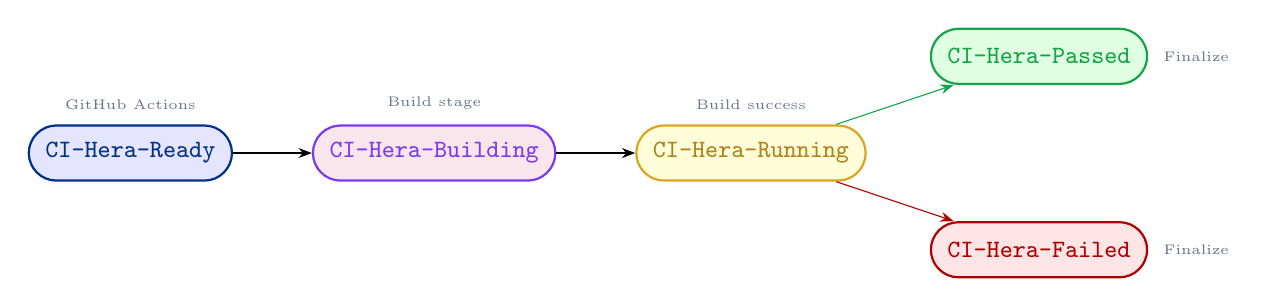
\begin{tikzpicture}[
  >=Stealth,
  lbl/.style={
    rectangle, rounded corners=10pt, minimum height=0.7cm,
    font=\small\ttfamily\bfseries, inner sep=6pt, draw, line width=0.8pt
  },
  every edge/.style={->, line width=1pt, gray}
]

\node[lbl, fill=blue!10, draw=noaablue, text=noaablue] (ready) {CI-Hera-Ready};
\node[lbl, fill=purple!10, draw=gitlabpurple, text=gitlabpurple,
  right=1cm of ready] (building) {CI-Hera-Building};
\node[lbl, fill=yellow!15, draw=Goldenrod, text=Goldenrod!80!black,
  right=1cm of building] (running) {CI-Hera-Running};
\node[lbl, fill=green!12, draw=vlabgreen, text=vlabgreen,
  above right=0.5cm and 0.8cm of running] (passed) {CI-Hera-Passed};
\node[lbl, fill=red!10, draw=red!70!black, text=red!70!black,
  below right=0.5cm and 0.8cm of running] (failed) {CI-Hera-Failed};

\draw[->] (ready) -- (building);
\draw[->] (building) -- (running);
\draw[->, vlabgreen] (running) -- (passed);
\draw[->, red!70!black] (running) -- (failed);

\node[font=\tiny\color{heragray}, above=2pt of ready]
  {GitHub Actions};
\node[font=\tiny\color{heragray}, above=2pt of building]
  {Build stage};
\node[font=\tiny\color{heragray}, above=2pt of running]
  {Build success};
\node[font=\tiny\color{heragray}, right=2pt of passed]
  {Finalize};
\node[font=\tiny\color{heragray}, right=2pt of failed]
  {Finalize};

\end{tikzpicture}
\end{adjustbox}
\caption{PR label state transitions through the CI pipeline lifecycle (Hera shown as example).}
\label{fig:label-lifecycle}
\end{figure}

When a test case fails, the \texttt{run\_check\_gitlab\_ci.sh} script
automatically posts a comment to the GitHub PR containing:
\begin{itemize}[leftmargin=1.5em]
  \item The failed case name and machine
  \item The experiment directory path
  \item Links to error log gists (uploaded via \texttt{publish\_logs.py})
\end{itemize}


% =============================================================================
\section{Nightly Pipeline Operations}
\label{sec:nightly}
% =============================================================================

Nightly pipelines are configured as \textbf{GitLab scheduled pipelines} with
\texttt{GFS\_CI\_RUN\_TYPE=nightly}. They differ from PR-triggered pipelines in
several ways.

\subsection{Directory Management}
\label{sec:nightly-dirs}

On successful completion of a nightly pipeline:

\begin{enumerate}[leftmargin=1.5em]
  \item The workspace directory is renamed from the pipeline-ID format to a
    date-based format:
    \begin{lstlisting}[style=bash, numbers=none]
# During execution:
${CI_BUILDS_DIR}/nightly_${CI_COMMIT_SHORT_SHA}_${CI_PIPELINE_ID}/

# After success:
${CI_BUILDS_DIR}/nightly_${CI_COMMIT_SHORT_SHA}_${MMDDYY}/
    \end{lstlisting}

  \item A \texttt{stable} symlink is created pointing to the latest successful
    nightly:
    \begin{lstlisting}[style=bash, numbers=none]
${CI_BUILDS_DIR}/stable -> nightly_${CI_COMMIT_SHORT_SHA}_${MMDDYY}/
    \end{lstlisting}

  \item Old nightly directories (except the stable target) are cleaned up.
\end{enumerate}

The \texttt{stable} directory is significant because CTest baseline data
(\texttt{STAGED\_CTESTS}) is sourced from it:

\begin{lstlisting}[style=bash, numbers=none]
export STAGED_CTESTS=${GITLAB_BUILDS_DIR}/stable/RUNTESTS
\end{lstlisting}

\subsection{Badge Updates}
\label{sec:badges}

Nightly pipelines update status badges stored as GitHub Gists. On success, a
green ``passed'' badge is generated; on failure, a red ``failed'' badge is
generated. These badges are referenced from the project README for visibility.

\begin{lstlisting}[style=bash, numbers=none]
# Badge generation (from finalize stage)
curl -sSL "https://img.shields.io/badge/${machine}_nightly-passed-brightgreen" \
  -o "${badge_img_file}"
${GH} gist edit "${badge_GIST_ID}" --add "${badge_img_file}"
\end{lstlisting}


% =============================================================================
\section{GitLab Runner Setup}
\label{sec:runners}
% =============================================================================

GitLab runners are deployed directly on each RDHPCS system. They execute as
\textbf{shell runners} (not Docker), running directly in the HPC environment
with access to the native compilers, Spack-Stack modules, and shared
filesystems.

\subsection{Platform Configuration Files}
\label{sec:platform-config}

Each supported platform has a configuration file at
\texttt{dev/ci/platforms/config.<MACHINE\_ID>} that defines platform-specific
paths and settings:

\begin{table}[H]
\centering
\caption{Platform Configurations}
\label{tab:platform-config}
\begin{tabularx}{\linewidth}{llX}
\toprule
\textbf{Platform} & \textbf{Config File} & \textbf{CI Root Directory} \\
\midrule
Hera & \texttt{config.hera} & {\small\texttt{/scratch3/NCEPDEV/global/\allowbreak role.glopara/GFS\_CI\_CD/HERA}} \\
Gaea\,C6 & \texttt{config.gaeac6} & {\small\texttt{/gpfs/f6/drsa-precip3/\allowbreak proj-shared/\$\{USER\}/GFS\_CI\_CD}} \\
Orion & \texttt{config.orion} & \texttt{/work2/noaa/global/\$\{USER\}/GFS\_CI\_CD/ORION} \\
Hercules & \texttt{config.hercules} & {\small\texttt{/work2/noaa/global/role-global/\allowbreak GFS\_CI\_CD/HERCULES}} \\
Ursa & \texttt{config.ursa} & {\small\texttt{/scratch3/NCEPDEV/global/\allowbreak role.glopara/GFS\_CI\_CD/URSA}} \\
WCOSS2 & \texttt{config.wcoss2} & {\small\texttt{/lfs/h2/emc/global/noscrub/\allowbreak globalworkflow.ci/GFS\_CI\_ROOT}} \\
\bottomrule
\end{tabularx}
\end{table}

Each configuration file exports the following key variables:

\begin{lstlisting}[style=bash, caption={Platform configuration variables (Hera example)}, label=lst:platform-vars, basicstyle=\ttfamily\footnotesize]
# Base directory for all CI operations
export GFS_CI_ROOT=/scratch3/NCEPDEV/global/role.glopara/GFS_CI_CD/HERA

# Initial condition data for experiments
export ICSDIR_ROOT=/scratch3/NCEPDEV/global/role.glopara/data/ICSDIR

# GitLab runner registration URL
export GITLAB_URL=https://vlab.noaa.gov/gitlab-community

# Human-readable runner name
export GITLAB_RUNNER_NAME="RDHPCS Hera"

# Directory where pipeline builds are stored
export GITLAB_BUILDS_DIR=${GFS_CI_ROOT}/BUILDS/GITLAB

# GitLab runner working directory (state files, config)
export GITLAB_RUNNER_DIR="${GFS_CI_ROOT}/GitLab/Runner"

# Baseline data for CTests
export STAGED_CTESTS=${GITLAB_BUILDS_DIR}/stable/RUNTESTS

# Custom Rocoto path (dry-run capable build)
export GFS_CI_ROCOTO_PATH="${GFS_CI_UTIL_PATH}/src/rocoto-1.3.7-dryrun_nodaemon/bin"
\end{lstlisting}

\begin{notebox}
Hera and Ursa share the same physical filesystem (cross-mounted), so their
\texttt{GFS\_CI\_ROOT} paths include the machine name (\texttt{HERA} or
\texttt{URSA}) to avoid collisions.
\end{notebox}

\subsection{The \texttt{launch\_gitlab\_runner.sh} Script}
\label{sec:launch-script}

The \texttt{dev/ci/scripts/utils/gitlab/launch\_gitlab\_runner.sh} script is the
primary tool for managing GitLab runners on each RDHPCS system. It supports
three operations: \textbf{register}, \textbf{run}, and \textbf{unregister}.

\subsubsection{Setup Prerequisites}

Before using the launch script, ensure:

\begin{enumerate}[leftmargin=1.5em]
  \item \textbf{Platform config exists}: A \texttt{config.<MACHINE\_ID>} file
    must exist in \texttt{dev/ci/platforms/} for the target machine.
  \item \textbf{Runner token is available}: The GitLab runner registration token
    must be available through one of:
    \begin{itemize}
      \item Command-line argument (second positional parameter)
      \item \texttt{GITLAB\_RUNNER\_TOKEN} environment variable
      \item A \texttt{gitlab\_token} file in the runner directory
    \end{itemize}
  \item \textbf{Runner binary}: The script will automatically download the
    GitLab runner binary if it is not present in the
    \texttt{GITLAB\_RUNNER\_DIR}.
\end{enumerate}

\subsubsection{Registering a Runner}

To register a new runner on an RDHPCS system:

\begin{lstlisting}[style=bash]
# SSH to the target HPC system
ssh role.glopara@hera.rdhpcs.noaa.gov

# Navigate to the global-workflow checkout
cd /path/to/global-workflow

# Register the runner (token can also be in GITLAB_RUNNER_TOKEN
# or gitlab_token file)
dev/ci/scripts/utils/gitlab/launch_gitlab_runner.sh register <GITLAB_RUNNER_TOKEN>
\end{lstlisting}

The registration command configures the runner with:
\begin{itemize}[leftmargin=1.5em]
  \item \textbf{Executor}: \texttt{shell} (runs directly in the HPC environment)
  \item \textbf{Shell}: \texttt{bash}
  \item \textbf{Builds directory}: \texttt{\$\{GITLAB\_BUILDS\_DIR\}} (from platform config)
  \item \textbf{Custom build directory}: enabled (allowing \texttt{.gitlab-ci.yml}
    to override the clone path via \texttt{GIT\_CLONE\_PATH})
  \item \textbf{Concurrency}: 24 concurrent requests
\end{itemize}

After registration, the script updates the runner's \texttt{config.toml} to set
\texttt{concurrent = 24}.

\subsubsection{Starting a Runner}

\begin{lstlisting}[style=bash]
dev/ci/scripts/utils/gitlab/launch_gitlab_runner.sh run
\end{lstlisting}

This launches the runner as a background process using \texttt{nohup}. The
runner's working directory is set to \texttt{\$\{GITLAB\_RUNNER\_DIR\}} from the
platform config. Logs are written to a date-stamped log file in the working
directory.

\subsubsection{Unregistering a Runner}

\begin{lstlisting}[style=bash]
dev/ci/scripts/utils/gitlab/launch_gitlab_runner.sh unregister
\end{lstlisting}

This removes the runner registration identified by
\texttt{\$\{GITLAB\_RUNNER\_NAME\}} from the GitLab server.

\subsection{Runner Directory Layout}
\label{sec:runner-layout}

Each platform follows a common directory structure under its
\texttt{GFS\_CI\_ROOT}:

% --- Figure 5: Directory tree ---
\begin{figure}[H]
\centering
\begin{tikzpicture}[
  every node/.style={font=\ttfamily\small, anchor=west},
  row/.style={yshift=-#1*0.45cm}
]
% Indentation helpers
\def\IA{0.4cm}    % indent level 1
\def\IB{0.8cm}    % indent level 2
\def\IC{1.2cm}    % indent level 3
\def\ID{1.6cm}    % indent level 4

% Root
\node[row=0] (r) {\$\{GFS\_CI\_ROOT\}/};

% BUILDS branch
\node[row=1] at (\IA,0) {\textcolor{noaadarkblue}{\rmfamily\textsf{\guilsinglright}}\; BUILDS/};
\node[row=2] at (\IB,0) {\textcolor{noaadarkblue}{\rmfamily\textsf{\guilsinglright}}\; GITLAB/};
\node[row=3] at (\IC,0) {\color{heragray}pr\_cases\_<sha>\_<id>/};
\node[row=4] at (\IC,0) {\color{heragray}nightly\_<sha>\_<date>/};
\node[row=5] at (\IC,0) {\color{vlabgreen}stable -> nightly\_<sha>\_<date>/};

% GitLab branch
\node[row=6] at (\IA,0) {\textcolor{noaadarkblue}{\rmfamily\textsf{\guilsinglright}}\; GitLab/};
\node[row=7] at (\IB,0) {\textcolor{noaadarkblue}{\rmfamily\textsf{\guilsinglright}}\; Runner/};
\node[row=8] at (\IC,0) (gr) {\color{heragray}gitlab-runner};
\node[row=9] at (\IC,0) (ct) {\color{heragray}config.toml};
\node[row=10] at (\IC,0) (gt) {\color{heragray}gitlab\_token};
\node[row=11] at (\IC,0) {\color{heragray}launched\_gitlab\_runner-*.log};

% Jenkins branch
\node[row=12] at (\IA,0) {\textcolor{noaadarkblue}{\rmfamily\textsf{\guilsinglright}}\; Jenkins/};
\node[row=13] at (\IB,0) {\color{heragray}agent/};
\node[row=14] at (\IB,0) {\color{heragray}workspace/};

% Annotations
\node[font=\rmfamily\itshape\scriptsize\color{heragray}, right=0.3cm of gr]
  {Runner binary};
\node[font=\rmfamily\itshape\scriptsize\color{heragray}, right=0.3cm of ct]
  {Runner configuration (auto-generated)};
\node[font=\rmfamily\itshape\scriptsize\color{heragray}, right=0.3cm of gt]
  {Optional token file};
\node[font=\rmfamily\itshape\scriptsize\color{heragray},
  anchor=west] at ($(r.east) + (0.3,0) + (0,-12*0.45cm)$)
  {Legacy};

% Tree lines
\draw[gray!50, line width=0.5pt]
  ([xshift=\IA-2pt, yshift=2pt]r.south west) -- ++(0, -14*0.45cm+0.2cm);
\draw[gray!50, line width=0.5pt]
  ([xshift=\IB-2pt]r.south west |- 0,-0.45cm) -- ++(0, -4*0.45cm+0.1cm);
\draw[gray!50, line width=0.5pt]
  ([xshift=\IB-2pt]r.south west |- 0,-6*0.45cm) -- ++(0, -5*0.45cm+0.1cm);
\draw[gray!50, line width=0.5pt]
  ([xshift=\IB-2pt]r.south west |- 0,-12*0.45cm) -- ++(0, -2*0.45cm+0.1cm);

\end{tikzpicture}
\caption{Runner directory layout on each RDHPCS platform.}
\label{fig:runner-layout}
\end{figure}

\subsection{Runner Maintenance}
\label{sec:runner-maint}

Common maintenance tasks:

\textbf{Check if a runner is active:}
\begin{lstlisting}[style=bash, numbers=none]
ps aux | grep gitlab-runner
\end{lstlisting}

\textbf{View runner logs:}
\begin{lstlisting}[style=bash, numbers=none]
tail -f ${GFS_CI_ROOT}/GitLab/Runner/launched_gitlab_runner-*.log
\end{lstlisting}

\textbf{Restart a runner} (e.g., after system maintenance):
\begin{lstlisting}[style=bash, numbers=none]
# Stop any existing runner
pkill -f "gitlab-runner run"

# Start fresh
cd /path/to/global-workflow
dev/ci/scripts/utils/gitlab/launch_gitlab_runner.sh run
\end{lstlisting}

\textbf{Re-register after token rotation:}
\begin{lstlisting}[style=bash, numbers=none]
# Unregister the old runner
dev/ci/scripts/utils/gitlab/launch_gitlab_runner.sh unregister

# Register with the new token
dev/ci/scripts/utils/gitlab/launch_gitlab_runner.sh register <NEW_TOKEN>

# Start the runner
dev/ci/scripts/utils/gitlab/launch_gitlab_runner.sh run
\end{lstlisting}


% =============================================================================
\section{Pipeline Execution Details}
\label{sec:execution}
% =============================================================================

\subsection{Build Stage}
\label{sec:build-stage}

The build stage (defined in \texttt{.build\_template} in
\texttt{.gitlab-ci.yml}) performs:

\begin{enumerate}[leftmargin=1.5em]
  \item \textbf{Environment setup}: Sources the platform config and validates
    paths.
  \item \textbf{Custom Rocoto loading}: If \texttt{GFS\_CI\_ROCOTO\_PATH} is set
    in the platform config, it is prepended to \texttt{PATH} to use a custom
    Rocoto build with dry-run support.
  \item \textbf{PR checkout}: For PR pipelines
    (\texttt{PR\_NUMBER\,!=\,0}), the build fetches the PR from GitHub and
    checks it out using \texttt{gh pr checkout}.
  \item \textbf{Build execution}: Calls
    \texttt{dev/ci/scripts/utils/ci\_utils.sh build}.
  \item \textbf{Workflow linking}: Runs \texttt{sorc/link\_workflow.sh} to
    create necessary symlinks.
  \item \textbf{Label updates}: Updates GitHub PR labels from
    \texttt{CI-<Machine>-Ready} to \texttt{CI-<Machine>-\allowbreak{}Building}
    and then to \texttt{CI-<Machine>-Running}.
\end{enumerate}

\subsection{Test Execution (PR Cases)}
\label{sec:test-pr}

The \texttt{run\_check\_gitlab\_ci.sh} script manages each experiment's
lifecycle:

\begin{enumerate}[leftmargin=1.5em]
  \item Launches the experiment with \texttt{rocotorun}.
  \item Enters a monitoring loop that alternates between \texttt{rocotorun}
    and \texttt{rocotostat} calls.
  \item Tracks Rocoto state through completion (\texttt{DONE}) or failure
    (\texttt{FAIL}, \texttt{UNAVAILABLE}, \texttt{UNKNOWN},
    \texttt{STALLED}).
  \item On failure: extracts error logs from failed/dead tasks, uploads them as
    GitHub Gists, and posts a comment to the PR.
  \item Exits with \texttt{rc=0} for success or \texttt{rc=1} for failure.
\end{enumerate}

% --- Figure 6: PR Case test execution flow ---
\begin{figure}[H]
\centering
\begin{adjustbox}{max width=\textwidth}
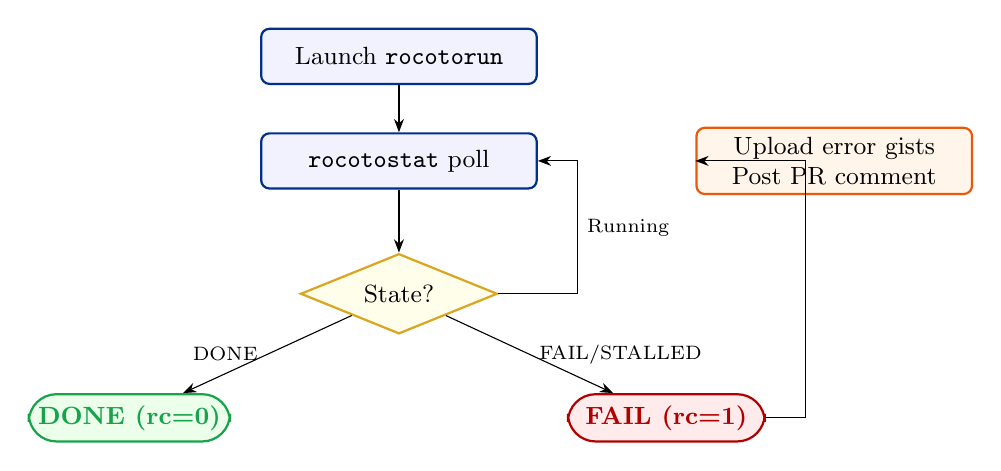
\begin{tikzpicture}[
  >=Stealth,
  node distance=0.6cm,
  proc/.style={
    rectangle, rounded corners=3pt, minimum width=3.5cm, minimum height=0.7cm,
    align=center, font=\small, draw=noaablue, line width=0.8pt, fill=blue!5
  },
  decision/.style={
    diamond, aspect=2, minimum width=2.5cm, align=center,
    font=\small, draw=Goldenrod, line width=0.8pt, fill=yellow!8
  },
  term/.style={
    rectangle, rounded corners=10pt, minimum width=2.5cm, minimum height=0.6cm,
    align=center, font=\small\bfseries, draw, line width=0.8pt
  }
]

\node[proc] (launch) {Launch \texttt{rocotorun}};
\node[proc, below=of launch] (stat) {\texttt{rocotostat} poll};
\node[decision, below=0.8cm of stat] (check) {State?};
\node[term, below left=1cm and 1.5cm of check, draw=vlabgreen,
  fill=green!8, text=vlabgreen] (done) {DONE (rc=0)};
\node[term, below right=1cm and 1.5cm of check, draw=red!70!black,
  fill=red!8, text=red!70!black] (fail) {FAIL (rc=1)};
\node[proc, right=2cm of stat, fill=orange!8, draw=triggerorg]
  (gist) {Upload error gists\\Post PR comment};

\draw[->] (launch) -- (stat);
\draw[->] (stat) -- (check);
\draw[->] (check) -- node[left, font=\scriptsize] {DONE} (done);
\draw[->] (check) -- node[right, font=\scriptsize] {FAIL/STALLED} (fail);
\draw[->] (check.east) -- ++(1,0) |- node[right, font=\scriptsize, pos=0.25]
  {Running} (stat.east);
\draw[->] (fail.east) -- ++(0.5,0) |- (gist);

\end{tikzpicture}
\end{adjustbox}
\caption{PR case test execution flow showing the Rocoto monitoring loop.}
\label{fig:pr-test-flow}
\end{figure}

\subsection{Test Execution (CTests)}
\label{sec:test-ctest}

CTest execution (defined in \texttt{.run\_ctests\_template} in
\texttt{gitlab-ci-ctests.yml}):

\begin{enumerate}[leftmargin=1.5em]
  \item Changes to the CTest build directory.
  \item Runs \texttt{ctest -L "\$\{CTEST\_NAME\}"} to execute tests for a
    specific label.
  \item Publishes JUnit XML results as GitLab artifacts.
  \item Examines both the \texttt{ctest} exit code and the JUnit XML for
    failure indicators.
\end{enumerate}

\subsection{Finalize Stage}
\label{sec:finalize}

On \textbf{success}:
\begin{itemize}[leftmargin=1.5em]
  \item PR pipelines: Adds \texttt{CI-<Machine>-Passed}, removes
    \texttt{CI-<Machine>-Running}.
  \item Nightly pipelines: Renames the workspace to date format, creates the
    \texttt{stable} symlink, cleans old directories, and updates status badges.
\end{itemize}

On \textbf{failure}:
\begin{itemize}[leftmargin=1.5em]
  \item PR pipelines: Adds \texttt{CI-<Machine>-Failed}, removes
    \texttt{CI-<Machine>-Running}.
  \item Nightly pipelines: Updates the status badge to show failure.
\end{itemize}

Failure cleanup is also handled in \texttt{after\_script} blocks that run
regardless of job status, canceling any remaining batch jobs and cleaning up
resources.


% =============================================================================
\section{Adding a New Host Platform}
\label{sec:new-host}
% =============================================================================

To extend the CI pipeline to a new RDHPCS system:

\begin{enumerate}[leftmargin=1.5em]
  \item \textbf{Create a platform config}: Add
    \texttt{dev/ci/platforms/config.<new\_machine>} with the required
    environment variables (follow an existing config as a template).

  \item \textbf{Define the test matrix}: Add a case matrix in
    \texttt{dev/ci/gitlab-ci-hosts.yml}:
    \begin{lstlisting}[style=yaml]
.new_machine_cases_matrix: &new_machine_cases
  - caseName: ["C48_ATM", "C48_S2SW", ...]
    \end{lstlisting}

  \item \textbf{Add host-specific jobs}: Create setup, run, and finalize jobs in
    \texttt{dev/ci/gitlab-ci-hosts.yml} that extend the appropriate templates
    and reference the new machine tag:
    \begin{lstlisting}[style=yaml, basicstyle=\ttfamily\footnotesize, xleftmargin=0pt]
setup_experiments-new_machine:
  extends: .setup_experiment_template
  variables:
    machine: new_machine
  tags:
    - new_machine
  parallel:
    matrix: *new_machine_cases
  needs:
    - build-new_machine
  rules:
    - if: $PIPELINE_TYPE == "pr_cases" && ...
    \end{lstlisting}

  \item \textbf{Add a build job}: Add a build job in
    \texttt{dev/ci/gitlab-ci-hosts.yml}:
    \begin{lstlisting}[style=yaml, basicstyle=\ttfamily\footnotesize, xleftmargin=0pt]
build-new_machine:
  extends: .build_template
  variables:
    machine: new_machine
  tags:
    - new_machine
    \end{lstlisting}

  \item \textbf{Register a runner}: SSH to the new machine and register
    a GitLab runner using \\
    \texttt{launch\_gitlab\_runner.sh register}.

  \item \textbf{Update GitHub Actions}: Add a new boolean input for the
    machine in \mbox{\texttt{.github/workflows/}}\linebreak
    \texttt{trigger-gitlab-pipelines.yml}.

  \item \textbf{Stage baseline data}: Ensure nightly baseline data is available
    at the \texttt{STAGED\_CTESTS} path for CTest validation.
\end{enumerate}


% =============================================================================
\section{File Reference}
\label{sec:file-ref}
% =============================================================================

\begin{longtable}{>{\raggedright\arraybackslash\small}p{6.8cm}p{7.7cm}}
\caption{Complete File Reference} \label{tab:file-ref} \\
\toprule
\textbf{File Path} & \textbf{Description} \\
\midrule
\endfirsthead
\toprule
\textbf{File Path} & \textbf{Description} \\
\midrule
\endhead
\bottomrule
\endfoot

\texttt{.gitlab-ci.yml} & Main pipeline orchestration and base templates \\
\texttt{dev/ci/gitlab-ci-cases.yml} & Setup, run, and finalize templates for experiment cases \\
\texttt{dev/ci/gitlab-ci-ctests.yml} & CMake/CTest setup and execution templates \\
\texttt{dev/ci/gitlab-ci-hosts.yml} & Per-host job definitions, test matrices, and runner tags \\
\texttt{dev/ci/platforms/config.*} & Platform-specific CI/CD environment configuration \\
\texttt{dev/ci/cases/pr/*.yaml} & Individual test case definitions (experiment YAML files) \\
\texttt{dev/ci/scripts/utils/ci\_utils.sh} & Core CI utility functions (build, create\_experiment, etc.) \\
\texttt{dev/ci/scripts/} \texttt{run\_check\_gitlab\_ci.sh} & Experiment monitoring, Rocoto polling, and failure reporting \\
\texttt{dev/ci/scripts/utils/gitlab/} \texttt{launch\_gitlab\_runner.sh} & GitLab runner registration, startup, and removal \\
\texttt{dev/ci/scripts/utils/gitlab/} \texttt{badge-updater-pipeline.yml} & Standalone badge update pipeline configuration \\
\texttt{dev/ci/scripts/utils/} \texttt{publish\_logs.py} & Error log upload to GitHub Gists \\
\texttt{dev/ci/scripts/utils/} \texttt{rocotostat.py} & Rocoto status parsing and reporting \\
\texttt{.github/workflows/} \texttt{trigger-gitlab-pipelines.yml} & GitHub Actions workflow for triggering GitLab pipelines \\

\end{longtable}


% =============================================================================
\section{Troubleshooting}
\label{sec:troubleshooting}
% =============================================================================

\subsection{Runner Not Picking Up Jobs}

\begin{enumerate}[leftmargin=1.5em]
  \item Verify the runner process is active:
    \texttt{ps aux | grep gitlab-runner}
  \item Check runner logs for connection errors.
  \item Ensure the runner tags match the job tags in the pipeline configuration.
  \item Verify network connectivity to the GitLab instance from the HPC node.
\end{enumerate}

\subsection{Build Failures}

\begin{enumerate}[leftmargin=1.5em]
  \item Check that \texttt{GW\_HOMEgfs} is correctly set and the directory exists.
  \item Verify that Spack-Stack modules are loadable on the target platform.
  \item Review the \texttt{ci\_utils.sh build} output in the job logs.
  \item For PR builds, ensure \texttt{gh} (GitHub CLI) is installed and
    authenticated.
\end{enumerate}

\subsection{Test Case Timeouts}

\begin{enumerate}[leftmargin=1.5em]
  \item Rocoto-based experiments have a maximum Rocoto cycle timeout configured
    in the CI runner (\texttt{RUNNER\_SCRIPT\_TIMEOUT: 8h}).
  \item If experiments consistently time out, check:
    \begin{itemize}
      \item Job scheduler queue availability on the HPC system.
      \item \texttt{maxtries} setting in the test case YAML.
      \item Whether batch jobs are being submitted and scheduled correctly.
    \end{itemize}
\end{enumerate}

\subsection{CTest Baseline Mismatches}

\begin{enumerate}[leftmargin=1.5em]
  \item Verify that \texttt{STAGED\_CTESTS} points to a valid, recent nightly build.
  \item Confirm the \texttt{stable} symlink is intact and pointing to a
    successful nightly.
  \item Check that the baseline data matches the current develop branch state.
\end{enumerate}

\subsection{GitLab Mirror Sync Issues}

\begin{enumerate}[leftmargin=1.5em]
  \item Verify the pull mirror is operational on the licensed GitLab instance
    (Settings $>$ Repository $>$ Mirroring repositories).
  \item Check the ``Last successful update'' timestamp --- it should be within the
    last few minutes.
  \item For push mirror issues to the community instance, verify the credentials
    and target URL are still valid.
  \item If a specific branch is missing, trigger a manual sync from the
    mirroring settings page.
\end{enumerate}


% =============================================================================
% Back matter
% =============================================================================
\vfill
\begin{center}
\rule{0.6\linewidth}{0.5pt}\\[6pt]
{\small\color{heragray}
  Document generated from the \texttt{gitlab\_documentation} branch of\\
  \texttt{NOAA-EMC/global-workflow} --- commit \texttt{fe77c911}\\[2pt]
  Synchronized with the \texttt{develop} branch as of March 2026.\\[4pt]
  NOAA / NWS / NCEP / EMC --- Global Workflow Development Team
}
\end{center}

\end{document}
